\documentclass{article}

\usepackage[ngerman]{babel}
\usepackage[T1]{fontenc}
\usepackage[utf8]{inputenc}
\usepackage{textcomp}
\usepackage{lmodern} %Type1-Schriftart für nicht-englische Texte
\usepackage{graphicx} %%Zum Laden von Grafiken
\usepackage{color} %für Farbmakierungen während der bearbeitung
\usepackage{url}

\begin{document}

\title{Geldwäsche und dessen Bekämpfung in der Bundesrepublik Deutschland}
\author{
    Autoren:\\
    sven.freiberg@haw-hamburg.de\\ 
    abdulhamid.cayirli@haw-hamburg.de\\
    david.gundermann@haw-hamburg.de\\
    fabian.stegemann@haw-hamburg.de\\
    abdessamed.aouam@haw-hamburg.de
}
\maketitle

\tableofcontents


\newpage

\part[Geldwäsche]{Geldwäsche}

    \section[Was ist Geldwäsche?]{Was ist Geldwäsche?}
            
        \subsection[Beschreibung]{Beschreibung}

            Als Geldwäsche wird das Einschleusen von Vermögenswerten, die aus einem Verbrechen oder aus bestimmten Straftaten herrühren (Vortaten), in den legalen Finanz- und Wirtschaftskreislauf, unter Verschleierung ihrer Herkunft, bezeichnet. Zu den Vortaten zählen z.B. Geldfälschung, Erpressung, Drogendelikte sowie Betrug, Korruption, organisierte Kriminalität, Terrorismus etc. Vortaten zur Geldwäsche werden durch lokale Gesetze definiert.
        
        \subsection[Zweck]{Zweck}

            Das wesensbildende Merkmal des Begriffs Geldwäsche besteht darin, dass der Ursprung der Vermögenswerte direkt oder indirekt auf eine kriminelle d.h. illegale und strafbare Handlung zurückzuführen ist.
            Der Geldwäsche verfolgt das Ziel, die unrechtmäßige Herkunft der Vermögenswerte zu verschleiern, um ihnen nach Durchlaufen verschiedener Transaktionen den Anschein der Rechtmäßigkeit zu geben. 
            Neben der bewussten Vertuschung der illegalen Herkunft geht es bei der Geldwäsche außerdem darum, die Beschlagnahme der unrechtmäßig erlangten Vermögenswerte durch die staatlichen Strafverfolgungsbehörden zu verhindern.

        \subsection[Ablauf]{Ablauf}

                Grundsätzlich werden 3 Stufen der Geldwäsche unterschieden, die einzeln oder zusammen auftreten und sich ggf. auch überschneiden können.

                \begin{enumerate}

                    \item Platzierung (Placement)

                        Unter der Platzierung (Placement) versteht man die Verschleierung der Herkunftsspuren des illegal erworbenen Geldes. Ferner soll die Identifikation sowie die Einziehung aus der kriminellen Tätigkeit durch den Staat verhindert werden. Die häufigsten Formen der Platzierung sind:
                        die zu verschleiernde Geldmenge wird in kleineren Teilbeträgen in der Regel ohne zeitlichen Zusammenhang auf Banken, Geldwechselstuben, Spielkasinos, Münzhändler oder Wertpapiermakler verteilt.
                        Investition des zu verschleiernden Geldbetrags in andere Vermögenswerte. Hierzu werden häufig Grundstücke, Luxusautos, Yachten, Schmuck etc. verwendet.
                        Darlehensgewährungen an von den Beteiligten der Vortat nahe stehende Personen, Personenvereinigungen oder Institutionen.
                        Beteiligungen an (stillen) Gesellschaften, die von den Beteiligten der Vortat beherrscht bzw. eingerichtet wurden.
                        Versteuerung als legal erwirtschaftete Umsätze in Betrieben, die den weiten Teil ihrer Umsätze mit Bargeld tätigen. Anfällig hierfür sind insbesondere der Gastronomiebereich, Taxibetriebe und auch In- und Exportfirmen.

                    \item Verteilung (Layering)

                        In der Stufe der Verteilung (Layering) werden die illegal erworbenen Geldbeträge in andere Staaten transferiert. Hierbei kommen folgende Begebenheiten im Ausland den Beteiligten an der Vortat zu Gute:
                        fehlende Buchführungspflicht,
                        fehlende Bankaufsicht,
                        mangelhafte Steuerkontrolle,
                        mangelhafte Strafvorschriften sowie
                        Vorhandensein von Domizil- und Finanzgesellschaften, welche kaum oder keinen Kontrollmechanismen unterliegen.
                        Beim Transfer des Geldes werden in der Regel unverdächtige Dritte (Anwälte, Treuhänder oder Scheinfirmen) zwischengeschaltet, die durch die länderspezifischen Finanzgeschäfte und eine Vielzahl von Transaktionen für Verwirrung sorgen und eine erschwerte Verfolgbarkeit der illegalen Erlöse nach sich ziehen. Dabei werden Berufsgeheimnis und Verschwiegenheitspflichten geschickt für die eigenen Zwecke eingesetzt.

                    \item Integration (Integration)

                        Durch die Maßnahmen der Beteiligten der Vortat im Rahmen der Integration (Integration) fließt das in der Herkunft verschleierte Geld in den legalen Wirtschaftskreislauf zurück und erhält einen legalen Anschein, als sei es auf rechtmäßigem und nachvollziehbarem Wege durch die Ausübung einer geschäftlichen Tätigkeit erworben worden. Auch hier bedienen sich die Täter der für die Geldwäsche besonders geeigneten Bargeldbetriebe, wie z.B. Taxibetriebe, Gastronomiebetriebe sowie Im- und Exportfirmen.
                        Bei der Rückführung des Kapitals in den legalen Wirtschaftskreislauf wird in der Regel auch eine Versteuerung hingenommen. Da der Geldwäscher im Allgemeinen eine gewinnbringende Anlage anstrebt, wird auch eine Steuerhinterziehung in Kauf genommen oder als Nebenziel angesehen.
                        Banken und Kreditinstitute spielen für alle 3 Stufen der Geldwäsche eine bedeutende Rolle. Garantierte Diskretion, Bank- und Berufsgeheimnis bieten unentbehrliche Vorteile für den Geldwäscher. Für eine Platzierung der Bargeldbeträge reicht schon eine Zwischenlagerung in Depots oder Bankschließfächern aus. Bankeigene Finanzdienstleistungen werden zur Verteilung benutzt und Darlehenstransaktionen, Akkreditive sowie die finanzielle Durchführung von Investitionsprojekten und die einfache Ausstellung von Schecks bietet den Geldwäschern Hilfestellung bei der Integration. Das Ganze erfolgt unter Ausnutzung der Stärken und Schwächen der Organisationsstrukturen und Überwachungsschwächen einzelner, für Geldwäsche besonders anfällige Länder.
                        Wichtigstes Hilfsmittel zur Bekämpfung der Geldwäsche sind die in vielen Ländern geltenden Schwellenwerte für Bargeldtransaktionen. Dies soll die Verteilung großer Mengen an Bargeld erschweren.

                \end{enumerate}
               
                \begin{figure}
                    \centering
                  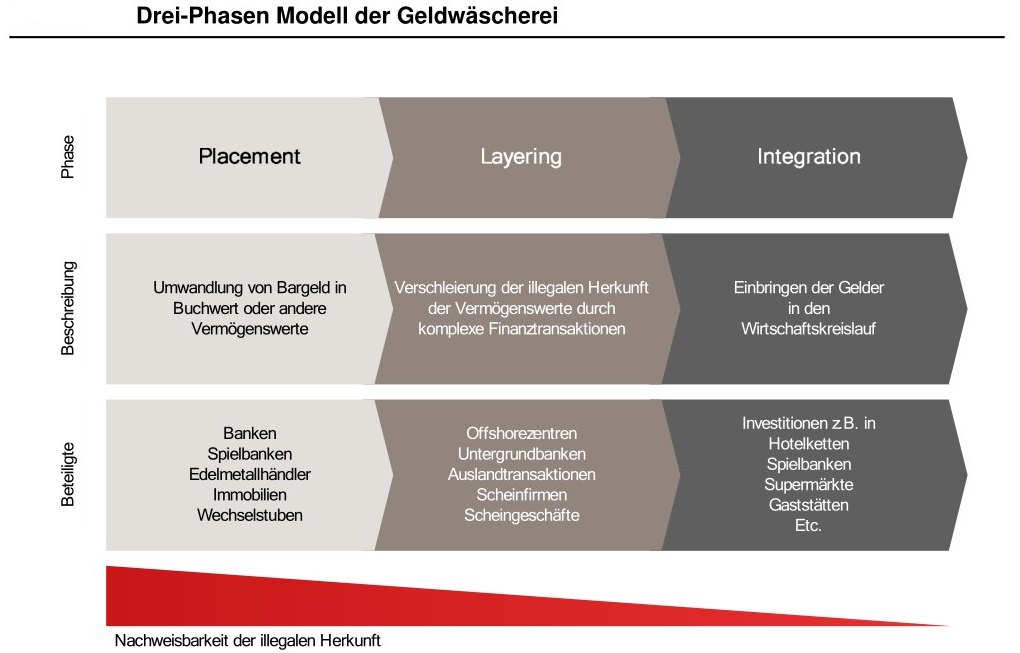
\includegraphics[scale=0.3]{../../turandon/data/drei_phasen_modell.png}
                    \caption{Drei-Phasen-Modell}
                    \label{fig2}
                                    \cite{Abb1}
                \end{figure}

        \subsection[Beispiel]{Beispiel}

            \texttt
            2012 ist der Goldverkauf in Italien aufgrund der schlechten Wirtschaftslage stark gestiegen.
            \cite{GoldItalien}
            Viele neue Goldhändler (einige kontrolliert von der Mafia) und Hinterhofgießerein und gründeten sich.
            Wenn ein Händler Gold im Wert von 1000 € verkauft und dem Käufer (gegen prozentualen Anteil) eine Quittung über 2000 € austellt, entsteht für den Händler ein Spielraum von knapp 1000 € um illegal erwirtschaftete Gelder mit in die Bücher des Geschäfts zu bringen.

\newpage

\part[Bekämpfung]{Geldwäschebekämpfung}

    \section[Beschreibung]{Beschreibung}

        Die wichtigste Grundlage in der Bekämpfung der Geldwäsche, ist die Transparenz von allen Beteiligten einer Geschäftsbeziehung oder eines Geldtransfers, sowie die Festellung der Herkunft der Finanzmittel.

        Zur Vorbeugung von Geldwäsche schreibt das Gesetz (Gesetz über das Aufspüren von Gewinnen aus schweren Straftaten bzw. GWG [Geldwäschegesetz]) bestimmte sogenannten Sorgfalten vor, welchen von allen im Gesetz erwähnten Verantwortlichen nachzukommen ist.

        Im Wesentlichenen gliedert sich die Bekämpfung in 2 Ebenen. Die erste ist die Vorsorge bzw. Sorgfalt des mit dem Geld handelnden Instituts. Sollte der Verantwortliche nicht in der Lage sein, allen unten genannten Punkten nachzukommen, ist die Geschäftsbeziehung unverzüglich zu beenden bzw. garnicht erst ein zu gehen. 
        Das zweite ist die durchgehende Dokumentation und das Archivieren der Transaktionen sowie möglicher weiterer Dokumente.

        \subsection[Transparenz des Geschäftspartners]{Transparenz des Geschäftspartners}

        \begin{enumerate}

            \item Identität

                Es sollen bei natürlichen Personen die Personendaten und bei juristischen Personen die Geschäftsdaten sowie der Vertreter festgehalten werden.

            \item Zweck und Art der Geschäftsbeziehung

                Der Verantwortliche muss Informationen über die Art der Geschäftsbeziehung sowie ihren Zweck vermerken, soweit dies nicht zweifelsfrei aus der Geschäftsbeziehung hervor geht.


            \item Prüfen über wirtschaftliche Berechtigung

                Eine natürliche Person ist dann wirtschaftlicher Berechtigter wenn sie mehr als 25 Prozent Kapitalanteile oder Stimmrechte des Betriebs hält.
                Weiterhin ist eine natürliche Person wirtschaftlich Berechtigter, falls sie unter der Kontroller des eigentlichen Geschäftpartners steht. Dies könnten z.B. Treuhänder oder Vermögensverwalter sein. In diesem Fall müssen zusätzlich die Daten des Vertretes des eigentlichen Geschäftspartners festgehalten werden.
                Auch kann es notwendig sein, zu überprüfen ob die verhandelnde Person eine politisch exponierten Person nahesteht oder selbst ein wichtiges öffentliches Amt ausübt. Sollte dies zutreffen, ist der Verantwortliche dazu aufgefordert die Geschäftsbeziehung verstärkten kontinuierlichen Überwachung zu unterziehen.

        \end{enumerate}           


        \subsection[Dokumentation der Geschäftsbeziehung]{Dokumentation der Geschäftsbeziehung}

        \begin{enumerate}

            \item Kontinuierliche Überwachung

                Der Veranwortliche muss während des Bestehens der Geschäftsbeziehungen oder unter besonderen Gesichtspunkten (siehe unten) alle Transaktionen dokumentieren. Auch soll transparent gemacht werden, woher die Vermögenswerte stammen, mit welchen der Verantwortliche arbeiten soll.
                Zusätzlich ist durchgängig festzuhalten, wie der Status der wirtschaftlichen Berechtigungen des Geschäftspartners oder eines Vertreters während der Geschäftsbeziehungen aussah.

            \item Archivierung

                Es geht aus dem GWG hervor, dass der Verantwortliche dazu verpflichtet ist, die Aufbewahrung der Unterlagen eines Zeitraums von mind. 5 Jahre sicherzustellen.
                Die Frist gilt jeweils ab Ende des Kalenderjahres des Abschlusses der Geschäftsbeziehung bzw. spätestens Ende des Kalenderjahres der Feststellung der Identität.
                Sammeln und dokumentieren von eingeholte Informationen, wie Identifikation oder Nachforschung sowie alle Transaktionen.

        \end{enumerate}  


        \subsection[Sonderfälle]{Sonderfälle}

        Es kann weiterhin Situationen außerhalb von bestehenden Geschäftsbeziehungen geben, in welchen es durch das GWG vorgeschrieben ist, den Sorgfaltspflichten nachzukommen oder - im schlimmsten Fall - eine Verdachtsmeldung abzusetzten. Diese beziehen sich auf folgende Punkte:

        \colorbox{red}{Eurozeichen im Text einheitlich gestalten Euro|€?}
        \begin{enumerate}

            \item Einzeltransaktionen

                Sollte es eine Transaktion von größer oder gleich 15000 € außerhalb einer Geschäftsbeziehung geben oder mehrere einzelne Transaktionen, bei denen Anhaltspunkte für eine unmittelbare Verbindung vorliegen und welche in Summe größer oder gleich 15000 € sind.

            \item Spielmarken

                Falls ein Kunde einer Spielbank oder eines Online-Glückspiels Marken im Wert von 2000€ oder mehr ein oder auszahlen ist auf jeden Fall dafür zu sorgen, dass der Kunde aussreichend identifieziert wird.

            \item Prämien bei Versicherungsvermittler

                Im falle von Prämienzahlungen in Bar, welche innerhalb eines Kalenderjahres den Wert von 15000€ übersteigen, muss der Vermittler Rückmeldung an sein Unternehmen geben, welches dann gegebenenfalls genannten Sorgfalten nach zu kommen hat.

            \item Begründeter Verdacht 

                Sollte der Verdacht naheliegen, dass die Finazmittel zur Terrorismusfinanzierung genutzt werden sollen oder es einen begründeten Verdacht gibt, dass die Finanzquelle von Straftaten herrührt.

            \item Zweifel an Identität

                Sollte es einen Verdacht an der Identität des Geschäftpartners geben.

            \item Zweifel an wirtschaftlicher Berechtigung

                Wenn es unklarheit gibt, ob der Geschäftspartner die notwendigen wirtschaftlichen Berechtigungen hat, um im Interesse seines Auftraggebers zu Handeln.

        \end{enumerate}    
    

    \section[Organe]{Organe}


        \subsection[Organe BRD]{Organe innerhalb der BRD}

            \begin{enumerate}

                \item Das Bundeskriminalamt (BKA)

                    Das BKA ist mit seiner Abteilung Zentralstelle für Verdachtsmeldungen bzw. der Financial Intelligence Unit (FUI) eine Bundesweite zentrale Anlaufstelle für Verdachstmeldungen der Geldwäsche oder Terrorismusfinanzierung, sofern es keinen anderen vorgeschriebenen Ansprechpartner laut GWG gibt.

                \item Bundesministerium der Finanzen (BdF)

                    Ist seit 2005 dazu berechtigt, Informationen zu einem Konto bei Kreditinstituen ein zu fordern, welche sich aber auf Stammdaten beschränkt und keine Auskunft über den eigentlichen Finanzverkehr beinhaltet. \cite{Tätigkeitsbericht}

                    Kann selbst oder in Zusammenarbeit mit BdI Umstände bzw Art und Weise von Meldungen in Form einer Verordnung bestimmen ohne den Bundesrat mit ein zu beziehen.

                \item Bundesministerium des Innern (BdI)

                    Kann in Zusammenarbeit mit BdF Umstände bzw Art und Weise von Meldungen in Form einer Verordnung bestimmen ohne den Bundesrat mit ein zu beziehen.                

                \item Finanzagentur GmbH das Bundesministerium der Finanzen

                    Ist zuständig für die Kreditanstalt für Wiederaufbau und die Bundesrepublik Deutschland.

                \item Bundesanstalt für Finanzdienstleistungsaufsicht (BaFin)

                    Die BaFin verfolgt das Ziel, einen Missbrauch des Finanzsystems zu Zwecken von Geldwäsche und Terrorfinanzierung zu verhindern. Sie sorgt dafür, dass die zu diesem Zweck bestehenden gesetzlichen Pflichten von den von ihr beaufsichtigten Unternehmen und Personen umgesetzt werden. Diese Pflichten ergeben sich aus dem Geldwäschegesetz (GwG), dem Kreditwesengesetz (KWG), dem Versicherungsaufsichtsgesetzt (VAG), dem Zahlungsdiensteaufsichtsgesetz (ZAG) oder dem Kapitalanlagegesetzbuch (KAGB). Schließlich ist in der Abteilung Geldwäscheprävention auch die elektronische Kontenabrufeinrichtung nach § 24c KWG angesiedelt. Hiermit können unter bestimmten Voraussetzungen Konten verdächtiger Terroristen oder anderer Straftäter bei in Deutschland ansässigen Kreditinstituten aufgespürt und an die jeweiligen Anfragenden (insbesondere Strafverfolgungsbehörden) übermittelt werden. Die Abteilung GW vertritt außerdem die finanzaufsichtlichen Interessen in diversen internationalen und europäischen Gremien, insbesondere in der Financial Action Task Force on Money Laundering (FATF) oder dem Sub-Committee on Anti Money Laundering (AMLC), einem Unterausschuss des Gemeinsamen Ausschuss der Europäischen Aufsichtsbehörden.
                   
                    Weiter Zuständigkeiten: 
                    \begin{enumerate}
                        \item
                            
                            Noch nicht abgedeckte Kreditinstitute mit Ausnahme der Deutschen Bundesbank

                        \item

                            Finanzdienstleistungsinstitute und Institute im Sinne des § 1 Absatz
                            2a des Zahlungsdiensteaufsichtsgesetzes.

                        \item

                            Im Inland gelegene Zweigstellen und Zweigniederlassungen von
                            Kreditinstituten, Finanzdienstleistungsinstituten und
                            Zahlungsinstituten mit Sitz im Ausland.

                        \item

                            Investmentaktiengesellschaften im Sinne des § 2 Absatz 5 des
                            Investmentgesetzes´.

                        \item

                            Kapitalanlagegesellschaften im Sinne des § 2 Absatz 6 des
                            Investmentgesetzes.

                        \item

                            Im Inland gelegene Zweigniederlassungen von EU-
                            Verwaltungsgesellschaften im Sinne des § 2 Absatz 6a des
                            Investmentgesetzes.

                        \item

                            Die Agenten und E-Geld-Agenten im Sinne des § 2 Absatz 1 Nummer 2b.

                        \item

                            Unternehmen und Personen im Sinne des § 2 Absatz 1 Nummer 2c.

                    \end{enumerate}

                \item Jeweils örtlich zuständige Aufsichtsbehörde für das Versicherungswesen

                    Verdachtsmeldungen von Versicherungsunternehmen und die im Inland gelegenen Niederlassungen solcher Unternehmen.

                \item Örtliche Rechtsanwaltskammer (§§ 60, 61 der Bundesrechtsanwaltsordnung)

                    Ist verantwortlich für die Meldungen von Rechtsanwälte und Kammerrechtsbeistände.

                \item  Patentsanwaltskammer (§ 53 der Patentanwaltsordnung)
                    
                    Verdachtsmeldungen von Patentanwälten.

                \item Präsident des Landgerichts, in dessen Bezirk der Notar seinen Sitz hat (§ 92 Nr. 1 der Bundesnotarordnung)

                    Meldungen von Notare des jeweiligen Bezirks.

                \item Wirtschaftsprüferkammer (§ 57 Abs. 2 Nr. 17 der Wirtschaftsprüferordnung)
                
                    Kümmert sich um Verdachtsmeldungen von Wirtschaftsprüfer und vereidigten Buchprüfer.

                \item Bundessteuerberaterkammer

                    Nimmt Verdachtsmeldungen von Steuerberater und Steuerbevollmächtigte entgegen.

            \end{enumerate}

        \subsection[Organe EU]{Organe der EU}

            \begin{enumerate}

                \item Financial Action Task Force (FATF)

                    Die FATF (Financial Action Tast Force on Money Laundering) versteht sich selbst als international führendes Gremium zur Bekämpfung der Geldwäsche und hat ihren
                    Sitz bei der OECD in Paris. Hauptziel der FATF ist die Entwicklung und Förderung von Grundsätzen zur Bekämpfung der Geldwäsche und der Terrorismusfinanzierung. Hierzu hat die FATF 40 Empfehlungen als Mindeststandards sowie 9 Sonderempfehlungen zur Bekämpfung der Terrorismusfinanzierung verabschiedet. Die FATF besteht gegenwärtig aus 34 Mitgliedsländern und 2 internationalen Organisationen.

                \item Europäischen Bankenaufsichtsbehörde 

                \item Europäischen Aufsichtsbehörde für das Versicherungswesen und die betriebliche Altersversorgung 

                \item Europäischen Wertpapier- und Marktaufsichtsbehörde 

            \end{enumerate}        

\newpage

    \section[Anmerkungen]{Anmerkungen}

        Obwohl es den Anschein macht, als habe es schon viele Bemühungen gegeben dem Probelm der Geldwäsche in der BRD Herr zu werden, gibt es wohl immer noch gewisse Versäumnisse was die Umsetzung der auf EU-Ebene beschlossenen Richtlinien anbetrifft. Folgend ein Fallbeispiel aus dem Jahr 2011.

        \subsection[Fallbeispiel]{Fallbeispiel}

            Durch die 2011 gefällte Entscheidung des Bundes, die Geldwäschebekämpfung seites der Überprüfung auf die Kommunen zu verlagen, ist die Regierung wohl davon aus gegangen, den EU-Richtlinien nun genüge getan zu haben.
            \begin{quote} Die Bundesregierung freut sich, der Europäischen Kommission mitteilen zu können, dass in allen Bundesländern die zuständigen Behörden (...) nunmehr bestimmt sind. \cite{EUZeugs} \end{quote}
            Dadurch entstehen solch bizzare Situationen, in welchen nun eine Standesbeamtin verantwortlich für die Überprüfung von hunderten Betrieben ist, die von Ausbildungswegen und Berufspraxis eigentlich garnicht dazu in der Lage ist diese durch zu führen. \begin{quote} Von Geldwäsche verstehe ich eigentlich gar nichts. ... Ja, kann man so sagen. \cite{Beatmin} \end{quote} Selbst wenn man dies ausser acht lässt, fehlt schlichtweg die Zeit um sich dieser Aufgabe zu stellen. Dadurch fehlt letztendlich die Überprüfende Instanz in den Betrieben, was die Kette der Geldwäschebekämpfung stark schwächt.

        \subsection[Ideen]{Ideen}

            Unserer Meinung nach, scheint es durchaus sinnvoll Überprüfende Instanzen auf Kommunaler ebene zu haben. Aber sollte dabei sichergestellt werden, dass es qualifiziertes Personal gibt. Ausserdem sollte darauf geachtet werden, genügend Arbeitzeit zur verfügung zu haben.

\newpage

    \begin{thebibliography}{9}

        \bibitem [1] {GoldItalien} \url{http://deutsche-wirtschafts-nachrichten.de/2012/08/20/wegen-krise-zahl-der-geschaefte-fuer-goldankaeufe-in-italien-hat-sich-vervierfacht/}, Stand: 06.01.2014

        \bibitem [2] {Tätigkeitsbericht} \url{http://www.sachsen-anhalt.de/index.php?id=20023}, Stand: 06.01.2014

        \bibitem [3] {EUZeugs} \url{http://www.wdr.de/tv/monitor/sendungen/2012/0908/pdf/geldwaesche.pdf}, Stand: 06.01.2014

        \bibitem [4] {Beatmin} Britt Paulsen, Verwaltungsbeamtin

        \bibitem [Wikipedia: BaFin] {bafin} \url{https://de.wikipedia.org/wiki/Bundesanstalt_f%C3%BCr_Finanzdienstleistungsaufsicht}, Stand: 06.01.2014

        \bibitem [Gesetz: GwG] {GwG} \url{http://www.gesetze-im-internet.de/gwg_2008/BJNR169010008.html}, Stand: 06.01.2014

        \bibitem [Abb1] {Abb1} \url{http://www.gap-consulting.eu/pdf/Kap4_Modell.pdf}, Stand: 06.01.2014
        
    \end{thebibliography}

\end{document}

